\documentclass{article}
\usepackage{graphicx} % Required for inserting images
\usepackage[colorlinks=true, allcolors=blue]{hyperref}
\usepackage{titlesec}
\usepackage{geometry}
 \geometry{
 a4paper,
 total={170mm,257mm},
 left=20mm,
 top=20mm,
 }
\graphicspath{ {./images/} }

\title{Unit 23}
\author{Chris}
\date{}

\begin{document}

\section{How cognitive computing can be used to help improve business activities}

\section{Healthcare}
Cognitive computing, is an evolving technology in healthcare augments the clinical thought process and enable the doctors to make the right diagnosis and preserve the patient's health in good condition. These systems provides timely care, optimal and cost-effective treatment. This highlighting hte platforms, techniques, tools, algortithms, applicationsk, and use case. This survey also explores about the works in the literature of present issues and prorpoese the future research directions of applying cognitive systmes in healthcare.


\section{Retail}
Cognitive computing has revolutionized the way enterprises operate and make decisions. By leveraging advanced technologies such as Artificial Intelligence (AI) and Machine Learning (ML), businesses can now harness the power of cognitive computing to streamline processes, enhance customer experiences, and gain valuable insights. Large Language Models (LLM) and Natural Language Processing (NLP) have revolutionized many use cases, enhancing productivity and experience. 

\section{Education}
The interactions between education and industry are a remarkable feature of cognitive computing, especially when it comes to its apllications in education and lesrning. Forexamle, complanies like IBM are using cognitive compuitn to harness the power of Big Data in multiple areas, including education.

\section{Finance}
Cognitive computing helps fiance by improving client-facing servces, future innovations and feasibility studies on innovation opportunities. How client-facing can improve with cognitive computer are doing provide innovative financial advisory solutions that would enable them to better serve their customers, and give them an edge in their competitive industry. How future innovations can improve with cognitive computing is by helping the client to understand the technology forecast adn where best to use them nad when it is eady to be used.

\section{Diagrams}
Diagram of cognitive computer in healthcare \\
\includegraphics[scale=0.5]{Healthcare} \\
Diagram of cognitive computing \\
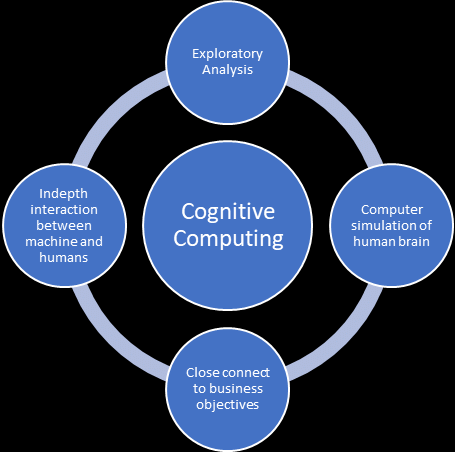
\includegraphics[scale=0.5]{Cognitive} \\

\break
\section{Source}
\href{Healthcare}{https://pubmed.ncbi.nlm.nih.gov/36990590/} \\
\href{Education}{https://blog.emb.global/cognitive-computing-in-education/} \\
\href{Finance}{https://www.linkedin.com/pulse/how-cognitive-computing-transform-finance-industry-naveen-joshi} \\

\end{document}
